\section{Turmeric}
\label{sec:turmeric}

\begin{spice}\label{spice:turmeric}
\textsc{Turmeric} \hfill \href{https://powo.science.kew.org/taxon/796451-1}{POWO} \\
\textbf{English:} \textit{turmeric}. 
\textbf{Arabic:} {\arabicfont{كركم}} \textit{kurkum}. 
\textbf{Chinese:} {\tradchinesefont{薑黃}} \textit{jiānghuáng} [ginger-yellow]; 黃薑 \textit{huángjiāng} [yellow-ginger]. 
\textbf{Hungarian:} \textit{kurkuma}.  \\
\noindent{\color{black}\rule[0.5ex]{\linewidth}{.5pt}}
\begin{tabular}{@{}p{0.25\linewidth}@{}p{0.75\linewidth}@{}}
Plant species: & \taxonn{Curcuma longa}{L.} (syn. \taxonn{Curcuma domestica}{Valeton}) \\
Family: & \textit{Zingiberaceae} \\
part used: & rhizome \\
Region of origin: & India \\
Cultivated in: & China; Honduras; India; Indonesia; Jamaica \\
Color: & orange-yellow \\
\end{tabular}
\end{spice}

\begin{figure}[!ht]
	\vspace{-4ex}
	\centering
	\subfloat{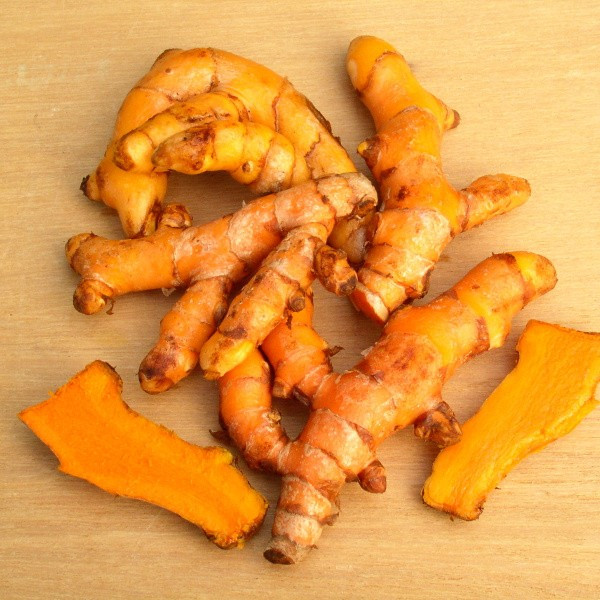
\includegraphics[width=0.3\linewidth]{imgs/spices/turmeric-4.jpg}}
	\hfill
	\subfloat{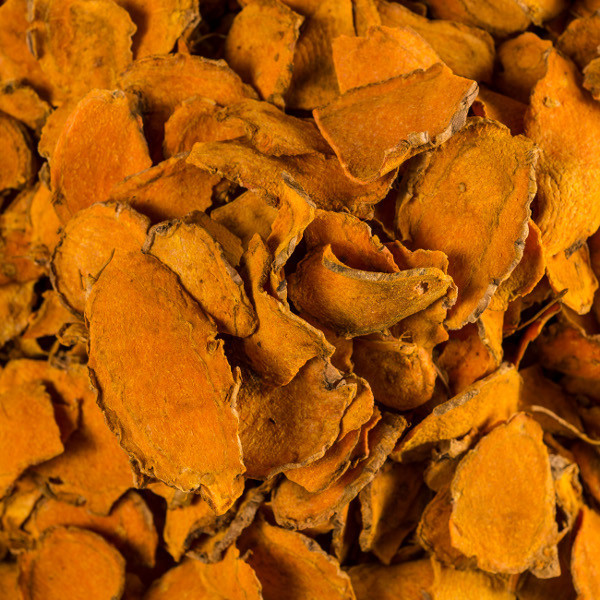
\includegraphics[width=0.3\linewidth]{imgs/spices/turmeric-1.jpg}}
	\hfill
	\subfloat{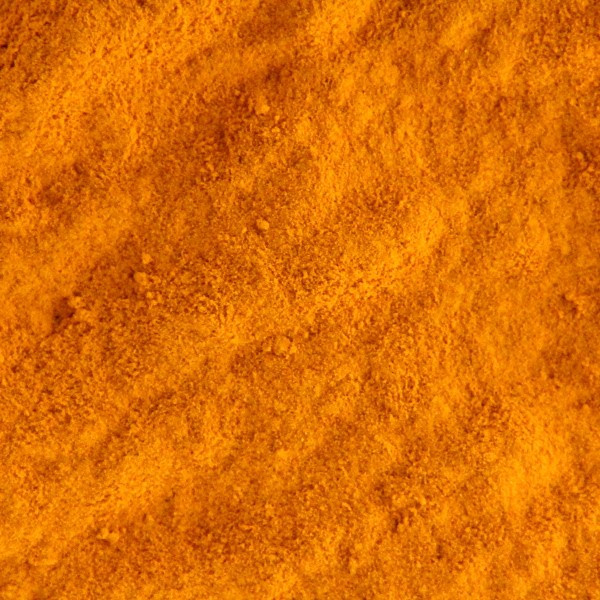
\includegraphics[width=0.3\linewidth]{imgs/spices/turmeric-3.jpg}}
	\caption{ \taxon{Curcuma longa}. Credits: Aromatiques.}
	\label{fig:turmeric_imgs}
\end{figure}

Turmeric is a spice obtained from the dried rhizomes of \taxon{Curcuma longa}, an aromatic plant closely related, and very similar to ginger. Commercial turmeric can be found in the shape of finger-like knobs, slices, and most commonly, powder. It can be seen on \cref{fig:turmeric_imgs}. Turmeric is an important ancient spice, medicine, dye, social and ritual substance, and it turns everything it touches yellow. It has a distinct smell and taste---it is slightly bitter and somewhat pungent---and it is used to color food, textiles, and even as a protection from evil spirits.\footnote{I have personally witnessed the practice of sprinkling turmeric on the doorstep of houses of the Indian community in Penang, Malaysia.} Tumeric, ``the golden spice'', is well known for its importance in South and Southeast Asian culinary traditions, (curries), traditional and modern medicine (\gls{Ayurveda}, see \textcite{prasad_turmeric_2011}), and religious traditions (e.g., \textit{haldi} ceremony before Hindu weddings; as blessing or \textit{prasad} `a benedictory material', see \textcite{nair_turmeric_2019}). Turmeric's color comes from curcumin, which is a coloring agent and common and approved food additive marked by the code E100 on regulated food products.

\subsection{The Botany, Origins, and Cultivation of Turmeric}


% Mabberley
% C. longa L. (C. domestica, turmeric, triploid cultigen orig. SE As.?) – dried & ground rhiz. (1 M t p.a. by 2013) used in curry powder & orange or yellow dyes form. much used with silk & wool, incl. in carpets, anti-oxidant, disinfectant (comm. plasters in Ind.), blocks 'tumour necrosis factor' that contributes to cancers & arthritis), pre-European introd. Polynesia & powder (mena) still integral part of med. & cerem. on Rotuma (Fiji); C. roscoeana Wall. (S As.) – imp. Thai cut-fl. export; C. zedoaria (Christm.) Roscoe ('C. zerumbet', zedoary, NE Ind.) – condiment or tonic, used in Ind. scents; others cult. orn.

\taxon{Curcuma longa} is a perennial herbaceous plant with large oblong leaves, short stem, and attractive white and yellow flowers that grow in clusters, from the ginger family \textit{Zingiberaceae} \autocite[128]{van_wyk_culinary_2014}. The plant is rhizomatous, meaning that the stems are subterranean, sending roots downwards, and shoots upwards. It is this rhizome that makes turmeric valuable as a spice, turning deeper and richer in color when dried.

Similarly to ginger, turmeric is an ancient sterile \gls{cultigen}, not found in the wild \autocite[128]{van_wyk_culinary_2014}. It does not produce seeds; it is propagated by splitting the rhizome. Therefore, as \textcite{kikusawa_proto_2007} points out, ``its distribution in the Pacific area is considered to obviously be the result of human introduction [...]'' Again, the origins of turmeric are not certain (and disputed), but it is believed to have been domesticated either in India \autocite{van_wyk_culinary_2014,powo,nair_turmeric_2019}, or Southeast Asia \autocite{mabberley_mabberleys_2017,kikusawa_proto_2007}. Turmeric needs a tropical climate to grow, it requires hight temperatures and rainfall. Harvesting means digging up the mature rhizomes that are then dried, sliced, and powdered \autocite[128]{van_wyk_culinary_2014}. The top producer of turmeric is India, but neighboring and Southeast Asian countries also cultivate and market turmeric as well.

Similarly used and botanically close plants include the paler yellow mango ginger (\taxon{C. amada}), the Indonesian mango ginger (\taxon{C. mangga}), wild turmeric (\taxon{C. aromatica}, also a dye), and zedoary (\taxon{C. zedoaria}), an alternative source for turmeric, especially in China \autocite[128]{van_wyk_culinary_2014}.




% WYK
% culinary uses Turmeric is best known as the spice that gives curry powder and mustard powder their bright orange or yellow colour. The fresh rhizomes, powdered rhizomes or extracts are important ingredients of Indian and Asian cooking. They are added to a wide range of dishes, not only for colour but also for flavour, including meat, fish, vegetables and rice dishes. A wellknown example is Malaysian yellow rice (nasi kunyit), eaten on ceremonial or festive occasions and the origin of the geelrys (“yellow rice”) of Cape cookery. Turmeric is used as a natural food dye in many food products, including mustard sauces, Worcestershire sauce, sandwich spread, butter, cheese, beverages, dairy products, drinks, confectionery, pickles and soup powders. Mango ginger has the flavour and aroma of raw mango and is used in curries and pickles.1 Indonesian mango ginger is similar to mango ginger in flavour and uses. Flavour compounDs The bright yellow colour is due to pigments (curcuminoids) of which curcumin is the main compound.3 The essential oil has a warm, spicy, earthy and slightly bitter flavour and contains mainly sesquiterpenes, of which ar-turmerone and turmerone are the major compounds.4 notes Curcumin has a wide range of medicinal properties.3

% 1. Nayar, N.M., Ravindran, P.N. 1995. Herb spices. In: Smartt, J., Simmonds, N.W. (Eds), Evolution of crop plants (2nd ed.), pp. 491–494. Longman, London. 2. Mabberley, D.J. 2008. Mabberley’s plant-book (3rd ed.). Cambridge University Press, Cambridge. 3. Esatbeyoglu, T., Huebbe, P., Ernst, I.M.A., Chin, D., Wagner, A.E., Rimbach, G. 2012. Curcumin—from molecule to biological function. Angewandte Chemie, International Edition, 51: 5308–5332. 4. Gopalan, B., Goto, M., Kodama, A., Hirose, T. 2000. Supercritical carbon dioxide extraction of turmeric (Curcuma longa). Journal of Agricultural and Food Chemistry 48: 2189.

% kikusawa_proto_2007

\subsection{The History of Turmeric}

Turmeric is widely used in South and Southeast Asia as a spice, medicine, cosmetic, and in rituals. In India, the use of turmeric dates back to Vedic period (c. 1500--c. 500 \BC). It is featured in the \gls{Sushruta}, the foundational text of traditional Indian medicine as an ingredient in a ointment for poisoned food \autocite{prasad_turmeric_2011}. The use of turmeric is most salient in the various island cultures of the Pacific, where it have spread with the Austronesian expansion around starting around 5000 \BP, reaching as far as Polynesia and Fiji, and used as a dye and ceremonial substance \autocite{mcclatchey_traditional_1993,sopher_indigenous_1964,prance_cultural_2005}. For the early history of turmeric, I recommend the book chapter titled \textit{Proto Who Utilized Turmeric, and How?} by \textcite{kikusawa_proto_2007}, which deals with the spread and uses of turmeric pre-European contact. It reached Tahiti, Hawaii, and the Easter Islands before the Europeans. Because of its role in Hindu rites, turmeric probably also spread to Southeast Asia at later stages as well, with the expansion of Hindu kingdoms in the region \autocite[170]{prance_cultural_2005}.

Turmeric, similarly to ginger, seems to have been known in Europe at early dates, but even if the modern identifications are correct, it was not a widespread substance before the \nth{7} century. ``There is no evidence of its use in the Levant and the Mediterranean Basin before the Islamic conquests.''---writes \textcite[108]{amar_arabian_2017}. In the \nth{1} century, Dioscorides noted in the \gls{DMM}: ``It is reported that there is also another kind of galingale that grows in India. It resembles ginger, it is saffron-colored and bitter when chewed, and it is a fast-acting depilatory when smeared on.'' \autocite{dioscorides_materia_2005}. Despite both Dioscorides and Pliny mentioning it, medieval Arabic authors considered it a novel spice not identified by the classic Greek authors \autocite[108]{amar_arabian_2017}. 
% According to \textcite{prance_cultural_2005}
% The spread of turmeric westward has been linked to the need of sun worshippers in Persia for more yellow dye than could be supplied by saffron. Turmeric was included among the coloring plants in an Assyrian herbal of the 6th century BC.

According to \textcite[2]{nair_turmeric_2019}, its maritime dispersion from India intensified in the Middle Ages, reaching the coast of China in the \nth{7} century \AD, and East Africa a century later, West Africa by 1200, and Jamaica in the \nth{18} century. In Chinese medicinal literature turmeric first appears in the \gls{Xinxiu}, and the \gls{Bencao} treats it as well \autocite{feng_molecular_2011}. 

From its initial diffusion up to Vasco da Gama's journey and landing in Kozhikode, it was Arab traders who were instrumental in the westward spread of turmeric, similarly to pepper and other spices of the time. It is said that in 1280, Marco Polo described turmeric in the China leg of his travels, but his vague description might agree with bastard saffron (safflower, \taxon{Carthamus tinctorius})\footnote{A plant introduced to China in the \nth{2} c. \BC from Western Asia \autocite[226]{polo_travels_1993}.}, or a species of \textit{Gardenia} that were used as yellow dye in East Asia at the time \autocite[226]{polo_travels_1993}.

\begin{quote}
	``There is also a vegetable which has all the properties of the true saffron, as well the smell as the colour, and yet it is not reall saffron. It is held in great estimation, and being an ingredient in all their dishes, it bears, on that account, a high price.'' \autocite[251-252]{komroff_travels_1926}
\end{quote}


% Turmeric derives its name from the Latin word terra merita, meaning meritorious earth, which refers to the color of ground turmeric, resembling a mineral pigment. The botanical name is Curcuma domestica Val. syn. Curcuma longa L. belongs to the family Zingiberaceae. The Latin name for turmeric is Curcuma longa, which has its origin in the Arabic name Kurkum, for this plant (Willamson 2002). In Sanskrit, it is called Haridra (“The Yellow One”), Gauri (“The One Whose Face Is Light and Shining”), Kanchani (“Golden Goddess”), and Aushadi (“Herb”). Haridra also comes from the Mundas, a pre-Aryan population, who lived through much of their life in northern India (Frawley and Lad 1993). The ancient Indian Vedas also refer to a set of people called Nishadas, literally translated as “Turmeric Eaters.” Turmeric has also been used as a dye for mustards, canned chicken broth, and pickles. It has been coded as food additive “E 100” in canned beverages, baked products, dairy, ice cream, yogurts, yellow cakes, biscuits, popcorn, sweets, cake icing, cereal, sauces, gelatin, and also direct compression tablets. Because of its unique color and history, turmeric has a special place in both Hindu and Buddhist religious ceremonies. Initially, it was cultivated as a dye because of its brilliant yellow color. With the passage of time, ancient populations came to know of its varied uses, and they began introducing it into cosmetics. The plant’s roots are used in one of the most popular Indian Ayurvedic preparations called Dashmularishta, a concoction prepared from ten different types of roots, which relieve fatigue, and have been in use since thousands of years. The plant’s flowers are used as an antidote against worms in the stomach of humans and can also cure jaundice and venereal diseases and have been known to have specific properties to combat mental disorders. Human breast tumors can be treated with turmeric leaf extracts.

% Today, turmeric is widely cultivated in the tropics and goes by different names in different cultures and countries (Table 13.1). In North India, turmeric is commonly called “haldi,” a word derived from the Sanskrit word haridra, and in the south it is called “manjal,” a word that is frequently used in ancient Tamil literature. The name turmeric derives from the Latin word terra merita (meritorious earth), referring to the color of ground turmeric, which resembles a mineral pigment. It is known as terre merite in French and simply as “yellow root” in many languages. In many cultures, its name is based on the Latin word curcuma. In Sanskrit, turmeric has at least 53 different names, including anestha (not offered for sacrifice or homa), bhadra (auspicious or lucky), bahula (plenty), dhirgharaja (long in appearance), gandhaplashika (which produces good smell), gauri (to make fair), gharshani (to rub), haldi (that draws attention to its bright color), haridra (dear to hari, Lord Krishna), harita (greenish), hemaragi (exhibits golden color), hemaragini (gives the golden color), hridayavilasini (gives delight to heart, charming), jayanti (one that wins over diseases), jawarantika (which cures fevers), kanchani (exhibits golden color), kaveri (harlot), krimighni or kashpa (killer of worms), kshamata (capability), laxmi (prosperity), mangalprada (who bestows auspiciousness), mangalya (auspicious), mehagni (killer of fat), nisha (night), nishakhya (known as night), nishawa (clears darkness and imparts color), patwaluka (perfumed powder), pavitra (holy), pinga (reddish-brown), pinja (yellow-red powder), pita (yellow), pitika (which gives yellow color), rabhangavasa (which dissolves fat), ranjani (which gives color), ratrimanika (as beautiful as moonlight), shifa (fibrous root), shobhna (brilliant color), shiva (gracious), shyama (dark colored), soubhagaya (lucky), survana (golden color), survanavara (which exhibits golden color), tamasini (beautiful as night), umavara (Parvati, wife of Lord Shiva), vairagi (who remains free from desires), varavarnini (which gives fair complexion), varna datri (enhancer of body complexion), varnini (which gives color), vishagni (killer of poison), yamini (night), yoshitapriya (beloved of wife), and yuvati (young girl).



\subsection{The Names of Turmeric}
\label{sec:names_of_turmeric}

\subsubsection{English}

\begin{etymology}\label{ety:turmeric}
English \textit{turmeric} `turmeric'
< French \textit{terre mérite} `turmeric'
< Medieval Latin \textit{terra merita} `turmeric'\footnote{}
\end{etymology}

According to most etymological dictionaries, the origins of \textit{turmeric} are obscure and uncertain.\footcites[turmeric]{oed}[turmeric]{oe}[turmeric]{ahd} However, they compare Medieval Latin \textit{terra merita}, and French \textit{terre mérite} meaning \textit{meritorious earth}, which according to \textcite[2]{nair_turmeric_2019} are the source, and refers to ``the color of ground turmeric, resembling a mineral pigment''---I consider this pure speculation. 

Truthfully, the English name of turmeric is probably the most obscure out of all English spice names. Dictionaries or authorities are only guessing, and even the immediate French and Latin etymons (\textit{terre mérite}; \textit{terra merita}) are speculative in terms of directionality. According to my readings, the latest attempt to explain the origins of the word \textit{turmeric} was published in an article by \textcite{guthrie_trade-language_2009}, who tried to tie the European word form to the trade languages of Northers India, for example Pashto \textit{tzer merich} [yellow pepper] (cf. Persian \textit{zard} `yellow', and Sanskrit \textit{marica} `[black] pepper'), but because of the lack of attestation in other languages or a continuous trail of linguistic evidence, I do not find this explanation convincing. Nevertheless, the author does a good job circumscribing the problematics of \textit{turmeric} and the previous attempts on solving it.

The term \textit{Indian saffron} tells us that Europeans who came into contact with turmeric first (most likely in Asia, as \textcite{nair_turmeric_2019} proposes mentioning Marco Polo) were reminded of saffron due to its similar use and coloring properties, and so this name was devised by compounding the geographic origin of the novel item with a prototype spice name based on their similarity in function. Arabic also uses a similar term as we will shortly see. 

It is worth pointing out that outside the United Kingdom, the whole of continental Europe uses derivations of (scientific) Latin \textit{curcuma}, or some other name not reminiscent of \textit{turmeric}. \textit{Curcuma}, besides being a botanical name for the genus is not used for turmeric in English, but it is connected to the Latin name of saffron, \textit{crocus}, which shows that the early confusion of the two names survives to this day in their binomial names. Both words go back to the Arabic etymon of \textit{kurkum}, which originally meant `saffron'.

\begin{table}[!ht]
\centering
\begin{tabularx}{\textwidth}{@{}l>{\itshape \small}lL>{\small}l@{}}
\toprule
\textbf{\#} & \multicolumn{1}{l}{\textbf{Species}} & \multicolumn{1}{l}{\textbf{Name}} & \multicolumn{1}{l}{\textbf{Source}} \\
\midrule
1	& Curcuma longa	& curcuma	& \textcite{oed} \\
2	& Curcuma longa	& Indian saffron	& \textcite{oed} \\
\textbf{3}	& \textbf{Curcuma longa}	& \textbf{turmeric}	& \textbf{\textcite{van_wyk_culinary_2014}} \\
\bottomrule
\end{tabularx}
\caption{Various names for turmeric in English.}
\label{table:names_turmeric_en}
\end{table}



% Nair
% The botanical name is Curcuma domestica Val. syn. Curcuma longa L. belongs to the family Zingiberaceae. The Latin name for turmeric is Curcuma longa, which has its origin in the Arabic name Kurkum, for this plant (Willamson 2002). In Sanskrit, it is called Haridra (“The Yellow One”), Gauri (“The One Whose Face Is Light and Shining”), Kanchani (“Golden Goddess”), and Aushadi (“Herb”). Haridra also comes from the Mundas, a pre-Aryan population, who lived through much of their life in northern India (Frawley and Lad 1993). The ancient Indian Vedas also refer to a set of people called Nishadas, literally translated as “Turmeric Eaters.” 

\subsubsection{Arabic}

\begin{etymology}\label{ety:kurkum}
\textbf{Arabic} {كركم} \textit{kurkum} `turmeric; saffron'; cf. cognates Hebrew \he{כַּרְכֹּום} \textit{karkom}; Aramaic \he{כּוּרְכְּמָא}/\sy{ܟܽܘܪܟܡܳܐ} \textit{kurkmā}; Akkadian \cu{𒌑𒆪𒄀𒆸𒈾} \textit{kurkanū}
<\textss{?} \textbf{Sanskrit} {कुङ्कुम } \textit{kuṅkuma} `saffron'\footnote{\textcite[s.v. kwrkm]{cal}; \textcite{guthrie_trade-language_2009}}
\end{etymology}
	
The Arabic word for turmeric is \textit{kurkum}, which originally meant `saffron'. The word \textit{kurkum} has a Hebrew cognate \textit{karkom}, and it appears in the Bible once,\footnote{Song of Songs 4:14 \url{https://www.biblegateway.com/passage/?search=Song\%20of\%20Songs\%204\%3A14\&version=NRSVUE}} together with other perfumes of ancient times, where it was identified as saffron. It is also generally accepted that this Semitic words is the etymon in the name of the saffron crocus, via the Greek word \gr{κρόκος} \textit{krókos}, found now in the Latin binomial name of saffron (\taxon{Crocus sativus}).

Arabic \textit{kurkum} has other Semitic (Aramaic, Akkadian), and regional cognates of Southwest Asia, such as Armenian \hy{քրքում} \textit{kʿrkʿum} (a loan from Syriac), Middle Perisan \textit{kwlkwm}, and it was suggested that this word originates in Sankrit, with an etymon of \textit{kuṅkuma} `saffron; saffron powder used as \textit{tilak}, a bright red dye used for marking forehead'.\footcite[164 \link{https://dsal.uchicago.edu/cgi-bin/app/soas_query.py?qs=ku\%E1\%B9\%85kuma\&searchhws=yes}]{turner_comparative_1962}. However, it might be the case that since these words originally mark saffron, native of the Eastern Mediterranean, it is actually the Sanskrit term that is ultimately derived from the Semitic, as claimed by \textcite{greppin_early_1987}. 
% Tibetan \ti{གུར་ཀུམ} is `safflower'.
According to \textcite[108]{amar_arabian_2017}, turmeric received the Semitic name (\textit{kurkum/karkom}) from saffron due to the close similarities of their main role: a yellow dye. They also say that this must have happened after the Islamic conquest of Arabia, which faciitated the introduction and diffusion of turmeric into the region. 

Just as in English, medieval Arabic literature called turmeric \textit{zaʿfarān hindī} `Indian saffron', and just as in Europe, turmeric in Arabia served as a cheap substitute for the extremely expensive saffron \autocite{amar_arabian_2017}.

% \sa{कुङ्कुम}
% \ar{زعفران هندي}

Further Arabic names include \textit{hurd} (in and around the Gulf, e.g., Yemen), via Persian \textit{hard}, most probably derived from the Sanskrit name of turmeric: \sa{हरिद्रा} \textit{haridrā} (cf. Hindi \hi{हल्दी} \textit{haldī}) \autocite{laufer_sino-iranica_1919}.

\begin{table}[!ht]
\centering
\begin{tabularx}{\textwidth}{@{}l>{\itshape \small}lr>{\itshape}lL>{\small}l@{}}
\toprule
\textbf{\#} & \multicolumn{1}{l}{\textbf{Species}} & \multicolumn{1}{l}{\textbf{Name}} & \multicolumn{1}{l}{\textbf{Tr.}} & \multicolumn{1}{l}{\textbf{Gloss}} & \multicolumn{1}{l}{\textbf{Source}} \\
\midrule
1	& Curcuma longa	& أصابع صفر	& aṣābiʿ ṣufr	& yellow fingers	& \textcite{wikipedia} \\
2	& Curcuma longa	& هرد	& hurd	& 	& \textcite{amar_arabian_2017} \\
\textbf{3}	& \textbf{Curcuma longa}	& \textbf{كركم}	& \textbf{kurkum}	& \textbf{phonetic}	& \textbf{\textcite{amar_arabian_2017}} \\
4	& Curcuma longa	& شجرة الخطاطيف	& shajarat al-khaṭāṭīf	& 	& \textcite{amar_arabian_2017} \\
5	& Curcuma longa	& زعفران هندي	& zaʿfarān hindī	& Indian saffron	& \textcite{amar_arabian_2017} \\
6	& Curcuma longa	& عقدة صفراء	& ʿuqda ṣafrā'	& yellow knob	& \textcite{baalbaki_-mawrid_1995} \\
7	& Curcuma longa	& عروق صفر	& ʿurūq ṣufr	& 	& \textcite{amar_arabian_2017} \\
\bottomrule
\end{tabularx}
\caption{Various names for turmeric in Arabic.}
\label{table:names_turmeric_ar}
\end{table}



\subsubsection{Chinese}

\begin{etymology}\label{ety:jianghuang}
\textbf{Mandarin Chinese} \traditionalchinesefont{薑黃} \textit{jiānghuáng} `turmeric', \textit{jiang} `ginger' + \textit{huang} `yellow'\footnote{\textcite[856]{kleeman_oxford_2010}}
\end{etymology}

In Chinese, turmeric today is known as \textit{jianghuang} [ginger-yellow], or less frequently as \textit{huangjiang} [yellow-ginger]. A historic name appearing in the \gls{Bencao} and reported by \textcite[312-313]{laufer_sino-iranica_1919} is used for both saffron and turmeric. More precisely, the \textit{yujin} [yü-gold] aromatic (\zh{香} \textit{xiang}) where the flowers are used (saffron), and the \textit{yujin} of the roots (turmeric, or some other \textit{Curcuma} species used similarly).

\begin{table}[!ht]
\centering
\begin{tabularx}{\textwidth}{@{}l>{\itshape \small}ll>{\itshape}lL>{\small}l@{}}
\toprule
\textbf{\#} & \multicolumn{1}{l}{\textbf{Species}} & \multicolumn{1}{l}{\textbf{Name}} & \multicolumn{1}{l}{\textbf{Tr.}} & \multicolumn{1}{l}{\textbf{Gloss}} & \multicolumn{1}{l}{\textbf{Source}} \\
\midrule
1	& Curcuma longa	& \tradchinesefont{寶鼎香}	& bǎodǐngxiāng	& treasure-cauldron-spice?	&  \\
2	& Curcuma longa	& \tradchinesefont{黃薑}	& huángjiāng	& yellow-ginger	& \textcite{defrancis_abc_2003} \\
\textbf{3}	& \textbf{Curcuma longa}	& \textbf{\tradchinesefont{薑黃}}	& \textbf{jiānghuáng}	& \textbf{ginger-yellow}	& \textbf{\textcite{kleeman_oxford_2010}} \\
\bottomrule
\end{tabularx}
\caption{Various names for turmeric in Chinese.}
\label{table:names_turmeric_zh}
\end{table}



\subsubsection{Summary}

\begin{table}[!ht]
\centering
\begin{tabularx}{\textwidth}{@{}ll>{\itshape}lLl>{\small}l@{}}
\toprule
\textbf{\#} & \textbf{Language} & \multicolumn{1}{l}{\textbf{Term}} & \textbf{Gloss} & \textbf{Loan} & \multicolumn{1}{l}{\textbf{Source}} \\
\midrule
1	& English	& curcuma	& 	& yes	& \textcite{oed} \\
2	& English	& Indian saffron	& 	& no	& \textcite{oed} \\
3	& English	& turmeric	& 	& yes	& \textcite{oed} \\
\midrule
1	& Arabic	& hurd	& 	& yes	& \textcite{lane_arabic-english_1863} \\
2	& Arabic	& kurkum	& phonetic	& yes	& \textcite{wehr_dictionary_1976} \\
3	& Arabic	& ʿuqda ṣafrā'	& yellow knob	& no	& \textcite{baalbaki_-mawrid_1995} \\
\midrule
1	& Chinese	& huángjiāng	& yellow-ginger	& no	& \textcite{defrancis_abc_2003} \\
2	& Chinese	& jiānghuáng	& ginger-yellow	& no	& \textcite{kleeman_oxford_2010} \\
\bottomrule
\end{tabularx}
\caption{Conventionalized names for turmeric in English, Arabic, and Chinese, found in dictionaries.}
\label{table:names_turmeric}
\end{table}

















% Cantonese: 黃薑 (wong4 goeng1)

% EE:
% (powder made from) the root-stock of the East Indian plant, used in curry powder, etc. XVI. Early forms also tarmaret, tormarith, which appear to be — F. terre mérite, modL. terra merita, of unkn. orig.; the ending shows assim. to -IC.

% OE:
% pungent powder made from the root of an East Indian plant, 1530s, altered from Middle English turmeryte (early 15c.), which is of uncertain origin. "Middle English Compendium" compares Medieval Latin terra merita (16c.), French terre mérite (17c.), literally "worthy earth," though the reason why it would be called this is obscure. Klein suggests it might be a folk-etymology corruption of Arabic kurkum "curcuma, saffron."

% MW:
% modification of Middle French terre merite saffron, from Medieval Latin terra merita, literally, deserving or deserved earth
% First Known Use: 15th century (sense 1a(1))

% AH:
% [Alteration of Middle English termeryte; akin to French terre mérite and New Latin terra merita, turmeric (New Latin, from Latin terra, earth; see ters- in the Appendix of Indo-European roots + merita, feminine past participle of merēre, to deserve; see (s)mer-2 in the Appendix of Indo-European roots).]

% WK:
% From Middle English turmeryte, tarmaret, of uncertain origin. Possibly from Old French terre mérite (“deserving earth”). According to Klein, possibly corrupted from Arabic كُرْكُم (kurkum, “Curcuma”). 